\documentclass[11pt]{article}
\usepackage{graphicx} % Required for inserting images
\usepackage[top=2.5cm, bottom=2.5cm, left=2.5cm, right=2.5cm]{geometry}
\usepackage[T1]{fontenc}
\usepackage{hyperref}
\usepackage[utf8]{inputenc}
\usepackage{multirow}
\usepackage{subcaption}
\usepackage{booktabs}
\usepackage{bookmark}
\usepackage{graphicx}
\usepackage{setspace}
\setlength{\parindent}{0in}
\usepackage{physics}
\usepackage{tikz}
\usepackage{tikz-3dplot}
\usepackage[outline]{contour} % glow around text
\usepackage{xcolor}
\usepackage{float}
\usepackage{makeidx}
\usepackage{fancyhdr}
\usepackage{pgfplots}
\usepackage{amsmath}
\pgfplotsset{compat=1.18}
\usepackage{caption}
\usepackage[english,catalan]{babel}
\setlength{\parskip}{11pt}
\usepackage{xcolor}
\usepackage{listings}
\usepackage{marginnote}
\usepackage{siunitx}
\usepackage{framed}
\usepackage{ulem}


\title{\Huge\bfseries Pràctica 6: \\ Feixos de raigs catòdics \\ [2ex] \Large}

\author{\begin{tabular}{c}
\textbf{GRUP A6} \\
Isaac Baldi García (1667260)\\
Miguel Ordejón de Prada (1710966) \\
Eira Jacas García (1666616) \\
Victor
\end{tabular}}

\date{Març 2025}

\begin{document}

\maketitle
\begin{center}
    \textbf{Abstract:} 
\end{center}


\newpage

\tableofcontents
\newpage

\section{Introducció Teòrica}

\section{Mètode Experimental}

\section{Desviació electroestàtica}\label{sec: desv_electr}

Teoria:
Una partícula de massa $m$ i càrrega $q$ sota l'influència d'un camp elèctric uniforme en direcció $y$ i magnitut $E$ i amb velocitat en direcció $x$ i magnitut $v_0$ descriurà la següent trajectòria:
\begin{align*}
    &x = v_0 t      &y = -\frac{qEt}{2m}
\end{align*}

Tenint en compte la conservació de la energia tenim:
\begin{equation*}
    \frac{1}{2}mv_0^2=qV_a
\end{equation*}

On $V_a$ és el potencial amb el que s'acceleren les partícules.

Y tenint en compte que el condensador de plaques planoparal·leles no és ideal:

Finalment, obtenim:
\begin{equation*}
    y = \frac{kV_px^2}{4dV_a}
\end{equation*}


Presentació de resultats:

--- Posar fotografies de la desviació electroestàtica ---

En subministrar una diferència de potencial a les plaques s'observa com el raig es desvia cap al càtode. Per tant, les partícules de les què està compost els raigs catòdics tenen una càrrega negativa.

 Les regressions lineals entre $y$ i $x^2$ confirmen que la trajectòria observada és una paràbola on els coeficients de correlació $R^2 \sim 0,98$ \footnote{Les regressions lineals en detall es troben a l'annex \ref{sec: traj_no_rect}}. D'aquestes també obtenim els diferents valors de k.

--- Gràfics amb incerteses ---
\begin{align*}
    V_p &= 1kV      & k = 0,905842781 \\
    V_p &= 2kV      & k = 1,392224283 \\
    V_p &= 3kV      & k = 2,131002674 \\
    V_p &= 4kV      & k = 2,42607494 
\end{align*}




\section{Desviació magnetoestàtica}\label{sec: desv_magn}
intro: Després de comprovar que les partícules dels ràigs catòdics tenen càrrega negativa (secció \ref{sec: desv_electr}) n'estudiem la interecció amb el camp magnètic, substancialment uniforme, generat per unes bobines de Hemholtz. 
El camp l'hem direccionat perpendicular als raigs catòdics i n'hem controlat la intencitat regulant la intencitat del corrent de les bobines. Al aplicar el camp, com era d'esperar, hem observat com els ràigs es corbaven i ens hem disposat a estudiar les dependències d'aquesta corba i el seu radi amb la intencitat del corrent de les bobines i amb el potencial dels raigs catòdics per poder determinar més propietats de les partícules d'aquests. 

Teoria: 
El camp d'inducció magnètica generat per unes bobines de Hemholtz es pot aproximar al camp uniforme 
\begin{equation}
    \vec{B}=\frac{32\pi nI}{5\sqrt{5}r}\cross10^{-7} \quad \hat{z}\quad Wb/m^2.
    \label{eq: B}
\end{equation}
Per la llei de Lorentz, una partícula carregada negativament sota un camp d'inducció magnètica, $\vec{B}$, pateix una força
\begin{equation}
    \vec{F}=q\vec{v}\cross\vec{B}.
    \label{eq: Lorentz} 
\end{equation} 
En el nostre cas, $\vec{v}$ és perpendicular a $\vec{B }$ i, per tant, les partícules dels raigs catòdics seguiran una trajectòria circular d'equació
%Aquesta força, al ser sempre perpendicular a la velocitat i tenint en compte que en el nostre sistema la velocitat de les partícules carregades, $\vec{v}$, és perpendicular a $\vec{B }$ induirà un moviment circular a les partícules de radi R. La trajectòria de les partícules carregades del nostre sistema complirà
\begin{equation}
    R=\frac{x^2+y^2}{2y}.
    \label{eq: radi}
\end{equation}
On R és el radi del cercle i hem agafag el centre de coordenades a la boca del tub de raigs catòdics i l'eix x del sistema paral·lel a la direcció de sortida dels raigs.

Igualant la força centrípeta a la força de Lorentz obtenim la relació 
\begin{equation}
    Bqv=\frac{mv^2}{R}
    \label{eq: fc=fl}
\end{equation}
que combinada amb l'equació \ref{eq: B} ens dona la relació entre el radi i la intencitat de corrent
\begin{equation}
    R=K\frac{1}{I} \quad on \quad K=\frac{mv5\sqrt{5}r}{32\pi n}\cross 10^7.
    \label{eq: IvsR}
\end{equation}
Tenint en compte l'equació \ref{eq: fc=fl} i la llei de la conservació de l'energia mecànica, $qV_a = \frac{1}{2}mv^2$, s'obté 
\begin{equation}
    \frac{q}{m}=\frac{2V_a }{B^2R^2}
    \label{eq: q/m}
\end{equation}
que ens permetrà calcular la relació $\frac{q}{m}$ de les partícules.

resultats:
Per calcular el radi de la trajectòria de les partícules dels raigs catòdics en funció de la intencitat de corrent de les bobines hem usat l'equació (\ref{eq: radi}) que defineix el radi com el pendent de la recta de regressió entre $x^2+y^2$ i $2y$. A la figura (\ref{fig: regressio_1}) hem representat algunes d'aquestes regressions i ja podem veure com a mesura que augmenta la intencitat, el pendent de la recta, és a dir el radi de les partícules, disminueix. 
\begin{figure}[H]
    \centering
    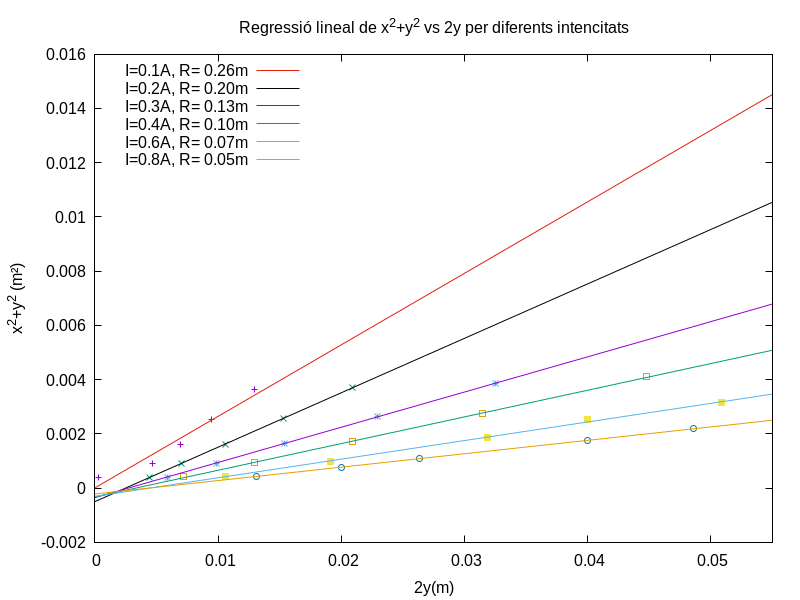
\includegraphics[scale=0.3]{regressio_1.png}
    \caption{Regressió per diverses intencitats de les bobines de Hemholtz de $x^2+y^2$ en front $2y$ on $y$ i $x$ són punts de la trajectòria dels raigs catòdics. La pendent de les rectes és el radi de corbatura de la trajectòria.}
    \label{fig: regressio_1}
\end{figure}

Agafant $0.1A, 0.2A, 0.3A, 0.4A, 0.5A, 0.6A, 0.7A, 0.8A$ com a intencitats de mostreig hem obtingut els radis de corbatura de la taula (\ref{tab:RvsI})\footnote{El càlcul de les incerteses es mostra a l'annex \ref{sec: incerteses}}. Amb aquestes dades (excloent l'última dada ja que té massa incertesa) hem construit la gràfica de la figura (\ref{fig: RvsI}) on es mostra que la variació de $R$ és lineal amb la variació de $\frac{1}{I}$. 
Al fer la regressió lineal del radi en funció de l'inversa de l'intencitat hem obtingut la recta
\begin{equation}
    y=x(0.03976\pm0.0006)+(0.0002\pm0.0016)
\end{equation}  
amb un coeficient de determinació de $r^2=0.99$ . Per tant, la relació és certament lineal i és compatible amb l'equació teòrica (\ref{eq: fc=fl}) ja que a més a més, l'ordenada a l'origen inclou el zero. El resultat de que $R$ és inversament proporcional a $I$ es producte de que al augmentar la intencitat de les bobines de Hemholtz el camp d'inducció magnètica augmenta provocant que les partícules rebin més força centrípeta què provoca la disminució del radi de la trajectòria.

 

\begin{figure}[h]
    \centering
    \begin{minipage}{0.45\textwidth}
        \centering
        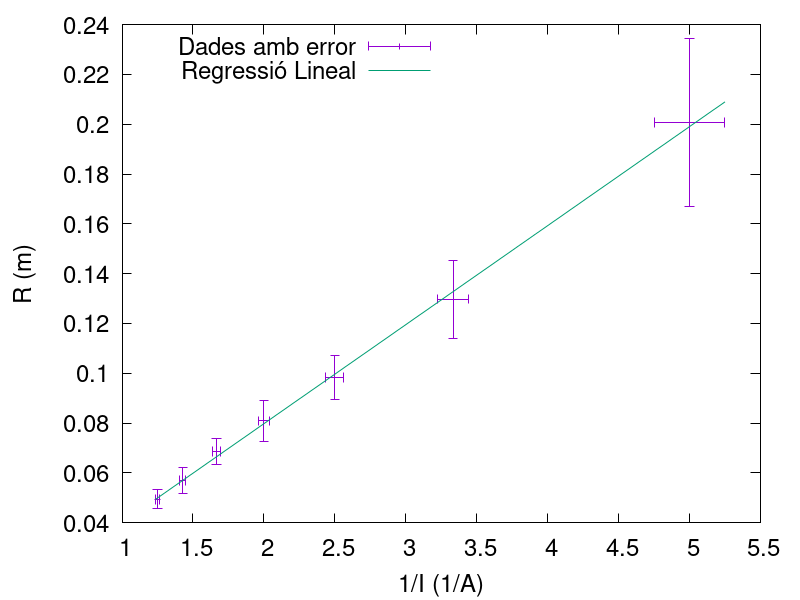
\includegraphics[width=\textwidth]{RvsI.png}
        \caption{Regressió de R en funció de $1/I$ excloent l'últim punt que perd la tendència.}
        \label{fig: RvsI}
    \end{minipage}
    \hfill
    \begin{minipage}{0.45\textwidth} 
        \centering
        \begin{tabular}{|c|c|}
            \hline
            I(A)	&	R (m)	\\\hline
            (0,800 ± 0,010)	&	(0,0494 ± 0,0037)	\\\hline
            (0,700 ± 0,010)	&	(0,0570± 0,0048)	\\\hline
            (0,600 ± 0,010)	&	(0,0685 ± 0,0051)	\\\hline
            (0,500 ± 0,010)	&	(0,0808± 0,0082)	\\\hline
            (0,400 ± 0,010)	&	(0,0983 ± 0,0089)	\\\hline
            (0,300 ± 0,010)	&	(0,1298 ± 0,016)	\\\hline
            (0,200 ± 0,010)	&	(0,201 ± 0,034)	\\\hline
            (0,100 ± 0,010)	&	(0,26 ± 0,10)	\\\hline
            
        \end{tabular}
        \captionof{table}{Resultats experimentals dels radis de la trajectòria per cada valor d'intencitat de corrent.}
        \label{tab:RvsI}
    \end{minipage}
\end{figure}



Per calcular el radi de la trajectòria de les partícules dels raigs catòdics en funció del potencial d'acceleració d'aquestes usem l'equació (\ref{eq: radi}) que defineix el radi com el pendent de la recta de regressió entre $x^2+y^2$ i $2y$. Agafant $2kV, 3kV, 4kV$ i $5kV$ com a potencials  de mostreig s'obtenen els radis de corbatura de la taula (\ref{tab:RvsVa}). Amb aquestes dades hem construit la gràfica de la figura (\ref{fig: RvsVa}) on es mostra que la variació de $R$ és cuadràtica amb la variació de $V_a$. AL fer la regressio lineal de $R^2$ respecte $V_a$ hem obtingut la recta
\begin{equation}
    y=x(2.93\times10^{-6}\pm0.27\times10^{-6})+(0.00228\pm0,00098)
\end{equation}  
amb un coeficient de determinació $r^2=0.98$. Per tant, la relació és certament lineal (cuadràtica respecte R) i compatible amb l'equació teòrica (\ref{eq: q/m}).

\begin{figure}[h]
    \centering
    \begin{minipage}{0.45\textwidth}
        \centering
        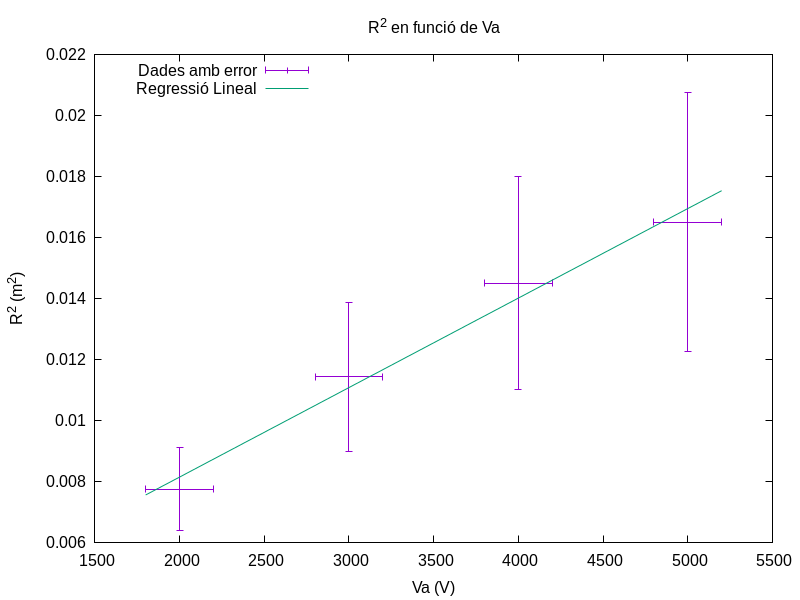
\includegraphics[width=\textwidth]{RvsVa.png}
        \caption{Regressió dels punts experimentals de $R^2$ en funció de $V_a$. Veiem que la relació és clarament lineal.}
        \label{fig: RvsVa}
    \end{minipage}
    \hfill
    \begin{minipage}{0.45\textwidth} 
        \centering
        \begin{tabular}{|c|c|}
            \hline
            Va (V)	&	R (m)	\\\hline
            (2000 ± 200)	&	(0.0880± 0.0077)	\\\hline
            (3000 ± 200)	&	(0.107± 0.011)	\\\hline
            (4000 ± 200)	&	(0.120± 0.014)	\\\hline
            (5000 ± 200)	&	(0.128 ± 0.015)	\\\hline
            
        \end{tabular}
        \captionof{table}{Resultats experimentals dels radis de la trajectòria per cada valor de potencial d'acceleració.}
        \label{tab:RvsVa}
    \end{minipage}
\end{figure}

Finalment, amb l'equació (\ref{eq: q/m}) i els resultats de tots els radis hem calculat que la relació q/m de les partícules dels raigs catòdics té un valor de 
\[
\boxed{\frac{q}{m}=(-4.16\pm0.88)\cross10^{11}\quad C/Kg.}
\]
Per fer-ho hem calculat la regressió lineal ajustada entre $2V_a$ i $B^2R^2$ i hem obtingut la recta $y=(4.16\pm0.38)x - (1412.64\pm791.71)$ amb un coeficient de determinació de $R^2=0.98$. El pendent d'aquesta recta ens ha donat el valor de q/m i després hem afegit l'incertesa instrumental al resultat. La linealitat dels punts indica que els nostres resultats concorden amb la teoria ja que com veiem a l'equació (\ref{eq: q/m}) la relació ha de ser lineal. Per altra banda si mirem la relació q/m dels electrons veiem que no és compatible amb el nostre resultat però sí que coincideix en ordre de magnitud. Això pot ser degut a que el camp magnètic generat per les bobines de Hemholtz no és uniforme fent que el seu valor difereixi del teòric.


\section{Desviació electromagnètica}\label{sec: desv_em}

En aquest tercer apartat ens interessem la relació càrrega/massa de les partícules dels raigs catòdics per a comprovar que aquesta coincideix amb la de l'electró. 

Tenint en compte el que ja hem pogut observar en els apartats anteriors: la desviació parabòlica a l'aplicar un camp elèctric E i desviació circular a l'aplicar el camp magnètic B, el que ens interessa en aquest tercer apartat és aplicant els camps de tal manera que de les dues deflexions estiguin al mateix pla però en amb direccions oposades. D'aquesta manera, aconseguim que la trajectòria dels raig catòdics no es vegi desviada, fet que ens permet igualar l forces elèctriques i magnètiques de tal manera quu arribem a la següent equació:

\begin{equation}\label{eq: Fm=Fe}
    qE = qvB
\end{equation}

amb la que es troba que la velocitat vindrà donada pel quocient

\begin{equation}
    v = \frac{E}{B}
\end{equation}

Podem obtenir el radi de la trajectòria circular deguda només a la desviació magnètica com s'explica a la secció \ref{sec: desv_magn}.

De les Eqs \eqref{eq: Fm=Fe}, I MES EQ (LA DEL RADI) es pot deduir l'equació que emprem per a calcular la relació càrrega/massa de la partícula que forma els raigs catòdics a partir de les nostres dades experimentals:

\begin{equation}
    \frac{q}{m}=\frac{E}{RB^2}=\frac{kV_p}{dK^2I^2R}
\end{equation}

Primerament, hem trobat el valor de la diferència de potencial aplicat entre les plaques amb el qual la desviació de la trajectòria rectilina paral·lela a l'eix de les abscisses és mínima\footnote{L'ampliació respecte aquest aspecte es troba en l'annex \ref{sec: traj_no_rect}}. 

En concret hem hagut d'aplicar una diferència de potencial $Vp = (0,85 + )$ kV per compensar un camp magnètic generat per bobines amb intensitat de $I = 100$ mA i un potencial $Va = 3$ kV per a l'accelaració de les partícules dels raigs catòdics.

En segon lloc, suprimint el camp elèctric $\vec{E}$ podem mesurar el radi de la trajectòria que deguda només de la desviació magnètica d'igual manera que en la secció \ref{sec: desv_magn}, el qual ha resultat ser $R = (A + A)$ m.

La constant del condensador $k$, la qual té en compte els efectes de vorada de les plaques, la podem obtenir com hem fet prèviament a la secció \ref{sec: desv_electr}. D'altra banda la constant de les bobines de Hemholtz $K$ ve determinada per la geometria d'aquestes, com s'explica en la secció \ref{sec: desv_magn}.

Per últim, un cop hem trobat la relació càrrega-massa q/m podem comparar-la amb la relació e/m, on e correspon a la càrrega d'un electró i m a la seva massa.

RESULTAT Q/M\footnote{El càlcul de les incerteses associades a aquest resultat es presenten en l'annex \ref{sec: inc_desv_em}}

\section{Conclusions}
les partícules eren indeed electrons!
\appendix{Annex}

\section{askdjfñla}

\section{Càlcul d'incerteses}\label{sec: incerteses}
\subsection{Desviació magnetoestàtica\label{sec: inc_desv_mag}}
\underline{Incertesa instrumental:} Hem agafat $\sigma_{c}=\pm0.01A$ i $\sigma_{t}=\pm100V$ com les incerteses de la font de corrent i la font de tensió respectivament. Per altra banda, hem agafat la mitjana del gruix del raig catòdic com  l'incertesa en la mesura dels punts de la trajectòria, ja que per trobar els punts hem usat un mètode de processat d'imatge molt exacte. Això d'ona una incertesa de les mesures de posició: $\sigma_{l}=\pm0.0014m$.

\underline{Propagació d'errors:} Per trobar les incerteses de magnituds dependents d'altres magnituds mesurables hem usat l'equació de propagació d'incerteses
\begin{equation}
    \sigma_{y}^2=\sum_{i=1}^{N}(\frac{\partial y}{\partial x_i})^2\sigma_{x_i}^2
\end{equation}
on y és la manitud dependent i ${x_i}$ les variables mesurables.
Per exemple, per l'incertesa del radi hem usat 
\begin{equation}
    \sigma_{R,ins}^2 = (\frac{\partial R(x,y)}{\partial x})^2 +(\frac{\partial R(x,y)}{\partial y})^2= \sigma_{l}^2\bigg[(\frac{x}{y})^2(1-\frac{(x^2+y^2)}{2y^2}^2)\bigg]
    \label{eq: ins_r}
\end{equation}
on hem agafat l'expressió del radi de l'equació \ref{eq: radi}.
En el cas del càlcul de l'incertesa dels radis, hem calculat l'incertesa combinada 
\begin{equation}
    \sigma_{R}=\sqrt{\sigma_{R,ins}^2+\sigma_{R,est}^2}
\end{equation}
on $\sigma_{R,ins}$ és l'incertesa instrumental trobada amb l'equació (\ref{eq: ins_r}) evaluada als valors mitjans de $y$ i $x$ de cada corba i $\sigma_{R,est}$ l'incertesa estadística del pendent calculada amb la regressió que hem usat per trobar el radi.

\subsection{Desviació electromagnètica}\label{sec: inc_desv_em}

\section{Trajectòria rectilinia amb camp elèctric i camp magnètic aplicat}\label{sec: traj_no_rect}

AFEGIR FOTOS!

Notem que aquesta trajectòria de fet, no és igual de rectílina a la trajectòria que podem observar quan no hi ha aplicat ni camp elèctric ni camp magnètic. Això és degut a la NO UNIFORMITAT DEL CAMP ELÈCTRIC (CONDENSADOR DE PLAQUES PETITES) I A LA NO UNIFORMITAT DEL CAMP MAGNÈTIC (SOLENOIDE NO PERFECTAMENT IDEAL).

\end{document}